\section{Date: 2024-09-30}
\noindent \textbf{Series ID: PRIICLAIMS} 

\noindent This series is titled Initial Claims in Puerto Rico and has a frequency of Weekly, Ending Saturday. The units are Number and the seasonal adjustment is Not Seasonally Adjusted.The observation start date is 1986-02-15 and the observation end date is 2024-09-21.The popularity of this series is 5. \\ 

\noindent \textbf{Series ID: WPU321101} 

\noindent This series is titled Producer Price Index by Commodity: Warehousing, Storage, and Related Services and has a frequency of Monthly. The units are Index Dec 2008=100 and the seasonal adjustment is Not Seasonally Adjusted.The observation start date is 2008-12-01 and the observation end date is 2024-08-01.The popularity of this series is 1. \\ 

\subsection{Regression Tables and Plots}
\begin{center}
\begin{tabular}{lclc}
\toprule
\textbf{Dep. Variable:}          & value\_fred\_WPU321101 & \textbf{  R-squared:         } &     0.028   \\
\textbf{Model:}                  &          OLS           & \textbf{  Adj. R-squared:    } &    -0.014   \\
\textbf{Method:}                 &     Least Squares      & \textbf{  F-statistic:       } &    0.6714   \\
\textbf{Date:}                   &    Mon, 30 Sep 2024    & \textbf{  Prob (F-statistic):} &    0.421    \\
\textbf{Time:}                   &        09:26:38        & \textbf{  Log-Likelihood:    } &   -101.43   \\
\textbf{No. Observations:}       &             25         & \textbf{  AIC:               } &     206.9   \\
\textbf{Df Residuals:}           &             23         & \textbf{  BIC:               } &     209.3   \\
\textbf{Df Model:}               &              1         & \textbf{                     } &             \\
\textbf{Covariance Type:}        &       nonrobust        & \textbf{                     } &             \\
\bottomrule
\end{tabular}
\begin{tabular}{lcccccc}
                                 & \textbf{coef} & \textbf{std err} & \textbf{t} & \textbf{P$> |$t$|$} & \textbf{[0.025} & \textbf{0.975]}  \\
\midrule
\textbf{const}                   &     113.9020  &        7.173     &    15.880  &         0.000        &       99.064    &      128.740     \\
\textbf{value\_fred\_PRIICLAIMS} &      -0.0026  &        0.003     &    -0.819  &         0.421        &       -0.009    &        0.004     \\
\bottomrule
\end{tabular}
\begin{tabular}{lclc}
\textbf{Omnibus:}       &  9.006 & \textbf{  Durbin-Watson:     } &    0.100  \\
\textbf{Prob(Omnibus):} &  0.011 & \textbf{  Jarque-Bera (JB):  } &    7.958  \\
\textbf{Skew:}          &  1.374 & \textbf{  Prob(JB):          } &   0.0187  \\
\textbf{Kurtosis:}      &  3.295 & \textbf{  Cond. No.          } & 5.66e+03  \\
\bottomrule
\end{tabular}
%\caption{OLS Regression Results}
\end{center}

Notes: \newline
 [1] Standard Errors assume that the covariance matrix of the errors is correctly specified. \newline
 [2] The condition number is large, 5.66e+03. This might indicate that there are \newline
 strong multicollinearity or other numerical problems.

\begin{figure}
\centering
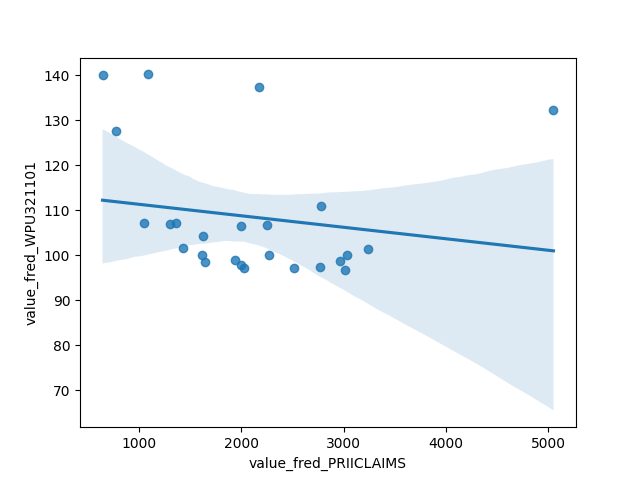
\includegraphics[scale = 0.9]{plots/plot_2024-09-30.png}
\caption{Regression Plot for 2024-09-30}
\end{figure}
\newpage
